
\subsection{Соединения серы, способы получения, химическое поведение, электронное и геометрическое строение молекул.}

\subsubsection*{$S_n$}

Аллотропия S:

- ромбическая $S_8$ - устойчивая\\
-моноклинная $S_8$\\
- пластическая $S_n$

\textbf{Способы получения}

1) Неполное сгорание $MeS$ и $H_2S$

$$MeS + O_2 \rightarrow MeO + S$$
$$H_2S + O_2 \rightarrow S + H_2O$$
$$H_2S + SO_2 \rightarrow S + H_2O$$

\textbf{Химические свойства}

1) С простыми веществами
$$S + O_2 \rightarrow SO_2$$
$$P + S \rightarrow P_2S_3$$
$$S+F_2 \rightarrow SF_6$$
$$Me + S \rightarrow MeS$$

2) Окисление

$$S + HClO_3 + H_2O \rightarrow H_2SO_4 + HCl$$

3) Образование поликатионов

$$S_8 + AsF_5 \rightarrow [S_8]^{2+}[AsF_6]_2^- + AsF_3(SO_2 liq)$$

4) Диспропорционирование

$$S + Na_2SO_3 \rightarrow Na_2S_2O_3$$
$$S + MeOH \rightarrow MeS + MeSO_3 + H_2O$$

\textbf{Электронное и геометрическое строение}

Устойчивые гомоцепи -S-S- (зигзагообразно)\\
$S_8$ - циклическая молекула, форма короны\\
Ромбическая - форма прямоугольного параллелепипеда;\\
моноклинная - скошенный параллелепипед;\\
пластическая - скрученные спиральные цепи.

\subsubsection*{$SO_2$}

\textbf{Способы получения}

$$S + O_2 \rightarrow SO_2$$
$$FeS + O_2 \rightarrow Fe_2O_3 + SO_2$$

\textbf{Химические свойства}

1) Высокая растворимость (40л $SO_2$ ы 1 л $H_2O$)
$$SO_2 + H_2O \leftrightarrows H_2SO_3$$

2) Горение

$$SO_2 + O_2 \rightarrow SO_3(400^{\circ},V_2O_5)$$

3) Восстановитель в щелочной среде
$$K_2CrO_4 + SO_2 + KOH + H_2O \rightarrow Cr(OH)_3 + K_2SO_4$$

4) Восстановитель в кислой среде

$$SO_2 + I_2 + H_2O \rightarrow HI + H_2SO_4$$
$$SO_2 + KMnO_4 + H_2O \rightarrow K_2SO_4 + MnSO_4 + H_2SO_4$$

5) Слабый окислитель в кислой среде 

$$SO_2 + HCl + FeC_2 \rightarrow FeCl_3 + H_2O + S$$

\textbf{Электронное и геометрическое строение}

Молекула изоэлектронна молекуле озона и имеет угловую форму

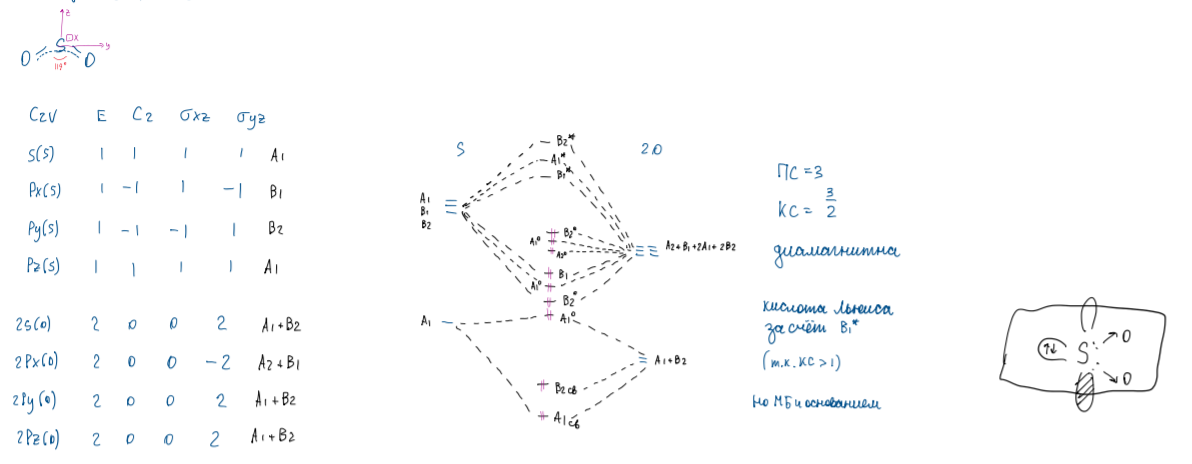
\includegraphics[scale=0.9]{images/7v1.png}

\subsubsection*{$SO_3$}

\textbf{Способы получения}

1) Горение $SO_2$

$$SO_2 + O_2 \rightarrow SO_3 (400^{\circ})$$
2) Распад (ди-)сульфатов

$$PbSO_4 \rightarrow PbO + SO_3 (900-1100^{\circ})$$
$$BaS_2O_7 \rightarrow BaSO_4 + SO_3$$

\textbf{Химические свойства}

1) Свойства кислотного оксида:

$$SO_3 + H_2O \rightarrow H_2SO_4$$

2) Окислительные свойства 

$$SO_3 + C \rightarrow SO_2 + CO_2$$
$$SO_3 + H_2S_{gas} \rightarrow SO_2 +S + H_2O$$
$$SO_3 + F_2 \rightarrow S_2O_6F_2(170^{\circ})$$

3) Легко реагирует с донорами $e^-$

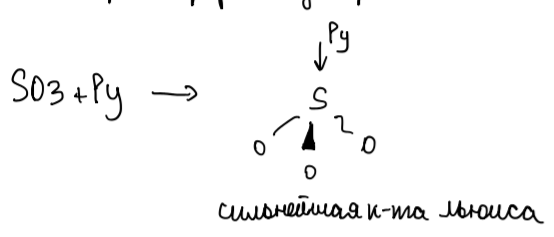
\includegraphics{images/7v2.png}

\textbf{Электронное строение}

Газообразное : плоский треугольник

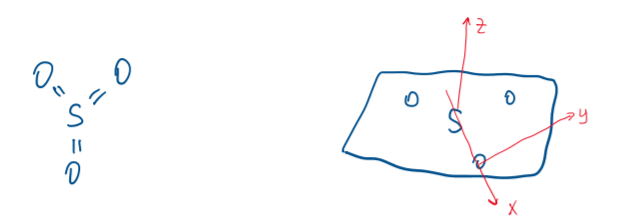
\includegraphics{images/7v3.png}

Кристалл - циклические тримеры $S_3O_9$ из тетраэдров $SO_4$ c общими вершинами

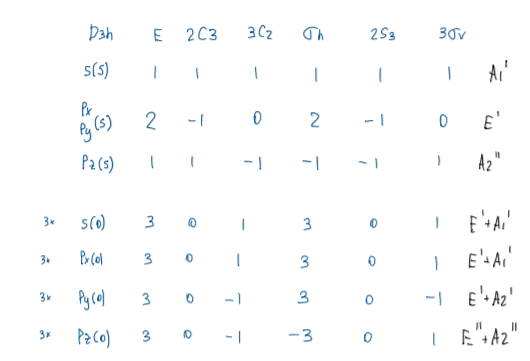
\includegraphics{images/7v4.png}\\
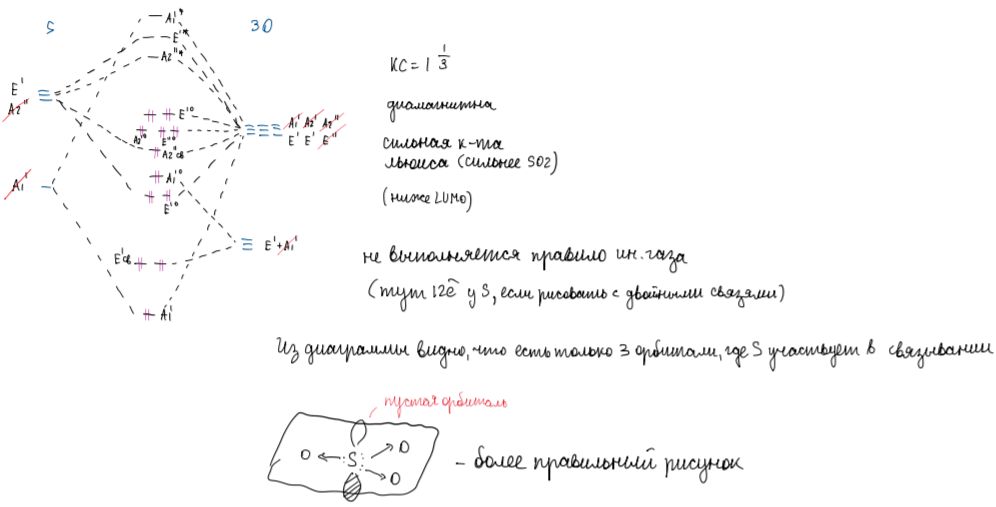
\includegraphics{images/7v5.png}

\subsubsection*{$H_2S$}

\textbf{Способы получения}

1) Реакции обмена
$$FeS + HCl \rightarrow FeCl_2 + H_2S$$

2) Гидролиз $CaS, BaS, Al_2S_3$

3) Из простых веществ

$$H_2 + S \rightarrow H_2S(600^{\circ})$$

\textbf{Химические свойства}

1) Слабая кислота в растворе

$$H_2S + CuSO_4 \rightarrow CuS\downarrow + H_2SO_4$$
$$NaOH + H_2S \rightarrow NaHS (Na_2S) + H_2O$$

2) Окисление $$H_2S + I_2 \rightarrow HI + S$$
$$H_2S + SO_2 \rightarrow S+ H_2O$$
$$H_2S + H_2SO_4 + KMnO_4 \rightarrow K_2SO_4 + H_2O + S$$
$$H_2S + O_2 \rightarrow SO_2 + H_2O$$

\textbf{Электронное и геометрическое строение}

Угловая молекула, полярна\\
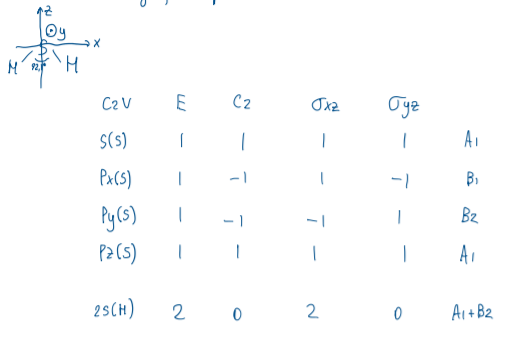
\includegraphics{images/6v4.png}
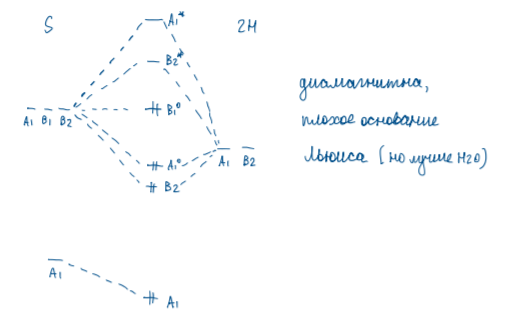
\includegraphics{images/6v5.png}

\subsubsection*{$H_2SO_3$}

\textbf{Способы получения}

 Устойчива только в растворе, в свободном состоянии не выделена

$$SO_2 + H_2O \leftrightarrows H_2SO_3$$

\textbf{Химические свойства}

1)Диссоциация по двум ступеням

2) Мягкий восстановитель

$$Fe_2(SO_4) + SO_2 + H_2O \rightarrow FeSO_4 + H_2SO_4$$

3) Соли - восстановительные свойства

$$SO_3^{2-} + O_2 \rightarrow  SO_4^{2-}$$

4) Разложение солей

$$MeSO_3 \rightarrow MeO + SO_2 (Me = Ca, Sr, Ba)$$
$$MeSO_3 \rightarrow Me_2SO_4 + Me_2S$$

\textbf{Электронное и геометрическое строение}

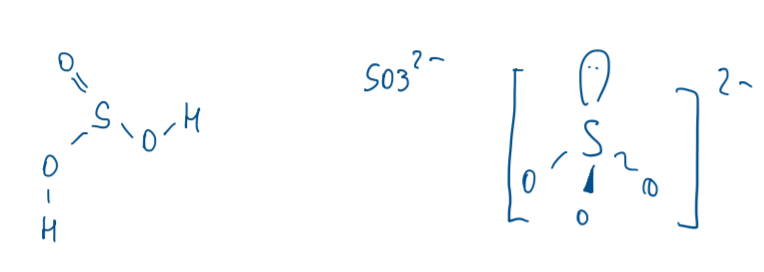
\includegraphics{images/7v6.png}

\subsubsection*{$H_2SO_4$}

\textbf{Способы получения}

Контактный способ:

$$SO_2 + O_2 \rightarrow SO_3(400^{\circ}, V_2O_5)$$
$$SO_3 + H_2O \rightarrow H_2SO_4$$
$$H_2SO_4 + SO_3 \rightarrow H_2SO_4\cdot SO_3$$
$$H_2SO_4\cdot SO_3 +H_2O \rightarrow H_2SO_4$$

\textbf{Химические свойства}

1) Сильная кислота

$$H_2SO_4 + H_2O \rightarrow H_3O^+ + HSO_4^-$$
$$HSO_4^- + H_2O \rightarrow H_3O^+ + SO_4^{2-}$$

2) Окислитель при $\omega > 70\%$

$$Zn + H_2SO_{4(konc)} \rightarrow ZnSO_4 + SO_2 + H_2O$$
$Fe,Cr, Al$ - при нагревании

3) Водоотнонимающее средство

$$KMnO_4 + H_2SO_4 \rightarrow Mn_2O_7 + KHSO_4 + H_2O$$

4) Соли обычно растворимы (кроме $Ba, Sr, Ca$)

$$CdSO_4 \rightarrow CdO + SO_3 (1400K)$$
$$Ag_2SO_4 \rightarrow Ag + SO_2 + O_2 (1050K)$$

\textbf{Электронное и геометрическое строение}

Тетраэдрическое окружение серы

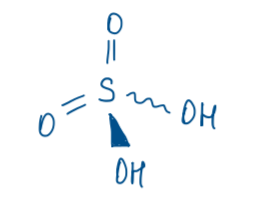
\includegraphics{images/7v7.png}


\subsubsection*{$H_2S_2O_3$ - тиосерная, $H_2S_2O_4$ - дитионистая .... $H_2S_nO_6$ - ди-,три-, политионовая}


\textbf{Способы получения}

Обычно кислоты не стойкие, существуют только в растворах

$$HSO_3Cl + H_2S \rightarrow H_2S_2O_3 + HCl$$
$$BaS_2O_4 + H_2SO_4 \rightarrow BaSO_4\downarrow + H_2S_2O_4$$
$$BaS_2O_6 + H_2SO_4 \rightarrow BaSO_4\downarrow + H_2S_3O_6$$

$$SO_2 + H_2S + NaOH \rightarrow Na_2S_2O_3 + H_2O$$
$$Na_2SO_3 + S \rightarrow Na_2S_2O_3$$
$$Zn + SO_2 \rightarrow ZnS_2O_4$$
$$MeO_2 + 2SO_2 \rightarrow Me_2S_2O_6 (Me= Mn, Ba)$$
$$Na_2S_2O_3 +I_2 \rightarrow Na_2S_4O_6 + NaI$$

\textbf{Химические свойства}

$$H_2S_2O_3 \rightarrow H_2O + SO_2 + S$$ 

Дитионаты - устойчивы, мягкие восстановители

$$Na_2S_2O_3 + I_2 \rightarrow Na_2S_4O_6 + NaI$$

Реакция лежит в основе иодометрии

Но: с сильными окислителями до $SO_4^{2-}$

$$Na_2S_2O_3 + Cl_2 + H_2O \rightarrow H_2SO_4 + NaCl + HCl$$

Комплексообразователи:

$$Na_2S_2O_4 + Fe_2(SO_4)_3 + H_2O \rightarrow FeSO_4 + Na_2SO_4 + H_2SO_4$$

$S_2O_6^{2-}$ - нет $red/ox$ свойств, используются, как инертные анионы.

$$BaS_2O_6 + H_2SO_4 \rightarrow BaSO_4\downarrow + H_2S_2O_6$$

Разложение:

$$H_2S_2O_6 \rightarrow H_2SO_4 + SO_2 (50^{\circ})$$
$$BaS_2O_6 \rightarrow BaSO_4 + SO_2$$

\textbf{Электронное и геометрическое строение}

Удобно рассматривать, как результат замещения $O$ или $OH^-$ на изоэлектронные частицы.

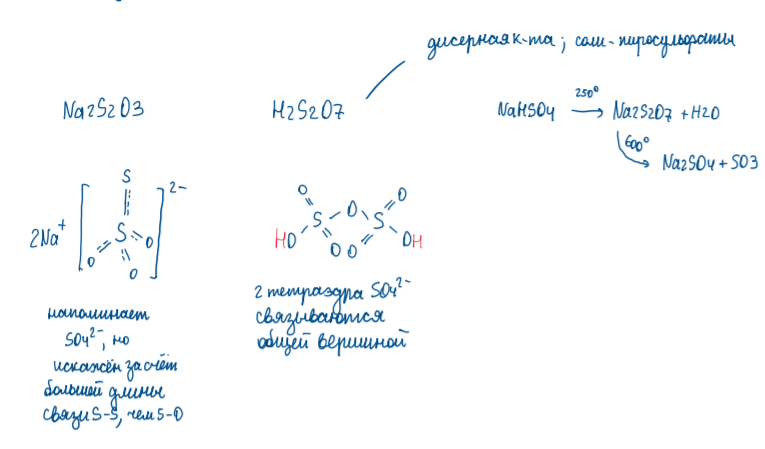
\includegraphics{images/7v8.png}

\subsubsection*{$H_2SO_5$ - кислота Каро (пероксомоносерная)}

\textbf{Способы получения}

$$H_2S_2O_8 + H_2O \rightarrow H_2SO_4 + H_2SO_5(0^{\circ})$$
$$H_2O_2 + HSO_3Cl \rightarrow H_2SO_5 + HCl$$

\textbf{Химические свойства}

1) Окислитель

$$H_2SO_5 + H_2O \rightarrow H_2SO_4 + H_2O_2$$

\textbf{Электронное и геометрическое строение}

Образуется при замене атома $O$ у $OH-$ группы в $H_2SO_4$ на перекисную группу

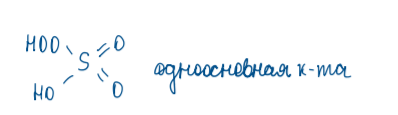
\includegraphics{images/7v9.png}

\subsubsection*{$H_2S_2O_8$ - пероксодисерная кислота}

\textbf{Способы получения}

1) Под действием электрического тока

$$H_2SO_4 \rightarrow H_2S_2O_8 + H_2$$
$$KHSO_4 \rightarrow K_2S_2O_8 + H_2$$

\textbf{Химические свойства}

1) Сильный окислитель

$$H_2S_2O_8 + H_2O + MnSO_4 \rightarrow HMnO_4 + H_2SO_4$$

2) Используется для получения $H_2O_2$

$$H_2S_2O_8 + H_2O \rightarrow H_2SO_4 + H_2O_2 (20^{\circ})$$

\textbf{Электронное и геометрическое строение}

Образуется при замене мостикового кислорода пиросерной кислоты на перекисную группу $-O-O-$

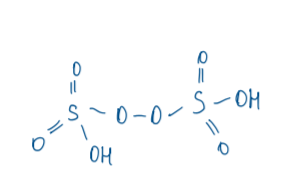
\includegraphics{images/7v10.png}

\subsubsection*{Галоленокислоты}

$HSO_3F$ - фторсульфоновая\\
$HSO_3Cl$ - хлорсульфоновая

\textbf{Способы получения}

$$SO_{2(liq.)} + HX \rightarrow HSO_3X(X=Cl,F)$$

\textbf{Химические свойства}

1) Очень сильные кислоты

2) С $H_2O_2$

$$HSO_3Cl + H_2O_2 \rightarrow H_2SO_5 + HCl$$

3) С $H_2S$ (до $HCl, H_2S_2O_3$ при $t<0^{\circ}$) 


\textbf{Электронное и геометрическое строение}

Получаются замещением $OH-$группы серной кислоты на изоэлектронные группы $Cl^-, F^-$

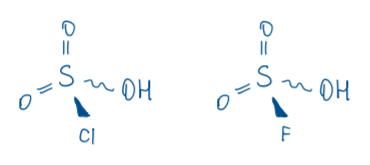
\includegraphics{images/7v11.png}
